\section{The Proposed Approach \label{sec-model}}

In this section, we present a \emph{H}eterogeneous network \emph{E}mbedding based  approach for \emph{Rec}emendation, called  \emph{HERec}.
For addressing the two issues introduced in Section 1, the proposed HERec approach consists of two major components.
First, we propose a new heterogeneous network embedding method to learn the user/item embeddings from HINs.
Then, we extend the classic matrix factorization framework by incorporating the learned embeddings using a flexible set of fusion functions.
We present an overall schematic illustration of the proposed approach in Fig.~\ref{fig_framework}.
After the construction of the HINs~(Fig.~\ref{fig_framework}(a)), two major steps are presented,  namely HIN embedding~(Fig.~\ref{fig_framework}(b)) and recommendation~(Fig.~\ref{fig_framework}(c)). Next, we will present detailed illustration of the proposed approach.

\subsection{Heterogeneous Network Embedding}
Inspired by the recent progress on network embedding~\cite{perozzi2014deepwalk,grover2016node2vec}, we adopt the representation learning method to extract and represent useful information of HINs for recommendation. Given a HIN $\mathcal{G} = \{\mathcal{V}, \mathcal{E}\}$, our goal is to learn a low-dimensional representation $\bm{e}_v \in \mathbb{R}^d$ (\aka embedding) for each node $v \in \mathcal{V}$.
The learned embeddings are expected to highly summarize informative characteristics, which are likely to be useful in recommender systems represented on HINs.
Compared with meta-path based similarity~\cite{sun2011pathsim,shi2015semantic}, it is much easier to use and integrate the learned representations in subsequent procedures.

However, most of the existing network embedding methods mainly focus on homogeneous networks, which are not able to effectively model heterogeneous networks. For instance, the pioneering study \emph{deepwalk}~\cite{perozzi2014deepwalk} uses random walk to generate node sequences, which
cannot discriminate nodes and edges with different types. Hence, it requires a more principled way to traverse the HINs and generate meaningful node sequences.

%In this section, we will present the details of heterogeneous network embedding. The basic idea is to employ a meta-path based random walk to generate a sequence of nodes, and then we maximize the co-occurrence probability of nodes to obtain the latent feature representation of nodes for one single meta-path, which reflect the structural characteristics of nodes from one perspective. Furthermore, we propose a flexible embedding fusion framework to combine the latent feature representation of nodes from different meta-paths.

\subsubsection{Meta-path based Random Walk}
To generate meaningful node sequences, the key is to design an effective walking strategy that is able to capture the complex semantics reflected in HINs. In the literature of HINs, meta-path is an important concept to characterize the semantic patterns for HINs~\cite{sun2011pathsim}.
Hence, we propose to use the meta-path based random walk method to generate node sequences. Giving a heterogeneous network $\mathcal{G} = \{\mathcal{V}, \mathcal{E}\}$ and a meta-path $\rho : A_1 \xrightarrow{R_1} \cdots A_t \xrightarrow{R_t} A_{t+1} \cdots \xrightarrow{R_l} A_{l+1}$, the walk path is generated according to the following distribution:

\begin{eqnarray}\label{eq-rw}
&&P({n_{t+1}=x |n_{t}=v, \rho})\\
&=&\begin{cases}
\frac{1}{|\mathcal{N}^{A_{t+1}}(v)|}, &\text{($v, x$) $\in$ $\mathcal{E}$ and $\phi(x) = A_{t+1}$};\nonumber\\
0,& \text{otherwise},
\end{cases}
\end{eqnarray}
where $n_t$ is the $t$-th node in the walk, $v$ has the type of $A_t$, and $\mathcal{N}^{(A_{t+1})}(v)$ is the first-order neighbor set for node $v$ with the type of $A_{t+1}$. A walk will follow the pattern of a meta-path repetitively until it reaches the pre-defined length.

\begin{exmp}
We still take Fig.~\ref{fig_framework}(a) as an example, which represents the heterogeneous information network of movie recommender systems.
Given a meta-path $UMU$, we can generate two sample walks (\ie node sequences) by starting with the user node of \emph{Tom}: (1) Tom$_{User}$ $\rightarrow$ The Terminator$_{Movie}$ $\rightarrow$  Mary$_{User}$, and (2) Tom$_{User}$ $\rightarrow$  Avater$_{Movie}$ $\rightarrow$  Bob$_{User}$ $\rightarrow$  The Terminator$_{Movie}$ $\rightarrow$  Mary$_{User}$. Similarly, given the meta-path $UMDMU$, we can also generate another node sequence: Tom$_{User}$ $\rightarrow$  The Terminator$_{Movie}$ $\rightarrow$  Cameron$_{Director}$  $\rightarrow$  Avater$_{Movie}$  $\rightarrow$ Mary$_{User}$. It is intuitive to see that these meta-paths can lead to meaningful node sequences corresponding to different semantic relations.
\end{exmp}

\begin{figure}[t]%[htbp]
\centering
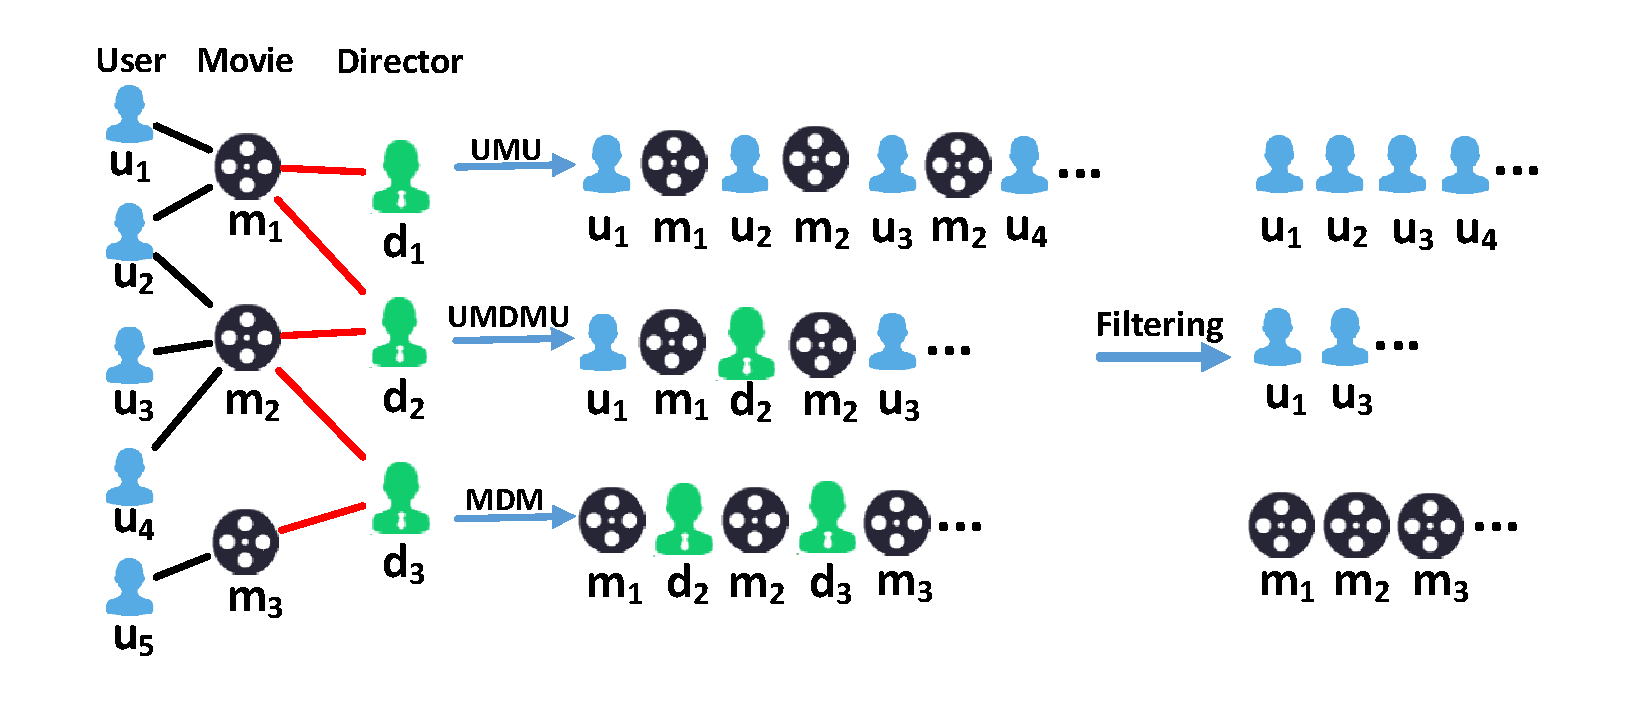
\includegraphics[width=9cm]{image/random_walk.pdf}
\caption{\label{fig_randwalk}An illustrative example of the proposed meta-path based random walk. We first perform random walks guided by some selected meta-paths, and then filter the node sequences \emph{not with} the user type or item type.}
\end{figure}

\subsubsection{Type Constraint and Filtering}
Since our goal is to improve the recommendation performance, the main focus is to learn effective representations for users and items,
while objects with other types are of less interest in our task.
Hence, we only select meta-paths starting with \emph{user type} or \emph{item type}.
Once a node sequence has been generated using the above method, it is likely to contain nodes with different types.
We further remove the nodes with a type different from the starting type.
In this way, the final sequence will only consist of nodes with the starting type.
Applying type filtering to node sequences has two benefits. First, although node sequences are constructed using meta-paths with heterogeneous types, the final representations
are learned using homogeneous neighborhood. We embed the nodes with the same type in the same space, which relaxes the challenging goal of representing all the heterogeneous objects in a unified space.
Second, given a fixed-length window, a node is able to utilize more homogeneous neighbors that are more likely to be relevant than others with different types.
%We present an illustrative example of the proposed meta-path random walk method in Fig. \ref{fig_randwalk}.

\begin{exmp}
As shown in Fig.~\ref{fig_randwalk}, in order to learn effective representations for users and items, we only consider the meta-paths in which the starting type is \emph{user type} or \emph{item type}. In this way, we can derive some meta-paths, such as $UMU$, $UMDMU$ and $MUM$.
 Take the meta-path of $UMU$ as an instance. We can generate a sampled sequence  ``$u_1 \rightarrow m_1 \rightarrow u_2 \rightarrow m_2 \rightarrow u_3 \rightarrow m_2 \rightarrow u_4$" according to Eq.~\ref{eq-rw}. Once a sequence has been constructed, we further remove the nodes with a different type compared with the starting node. In this way, we finally obtain a homogeneous node sequence ``$u_1 \rightarrow u_2 \rightarrow u_3 \rightarrow u_4$".
\end{exmp}

 The connections between homogeneous nodes are essentially constructed via the heterogeneous neighborhood nodes. After this step, our next focus will be how to learn effective representations for homogeneous sequences.

\subsubsection{Optimization Objective}
Given a meta-path, we can construct the neighborhood $\mathcal{N}_u$ for node $u$ based on co-occurrence in a fixed-length window.
Following node2vec~\cite{grover2016node2vec}, we can learn the representations of nodes to optimize the following objective:
\begin{equation}
\max_f \sum_{u \in \mathcal{V}}{\log Pr(\mathcal{N}_u | f(u))},
\end{equation}
where $f: \mathcal{V} \rightarrow \mathbb{R}^d$ is a function (aiming to learn) mapping each node to $d$-dimensional feature space, and $\mathcal{N}_u  \subset \mathcal{V}$ represents the neighborhood of node $u$, \emph{w.r.t.} a specific meta-path. We can learn the embedding mapping function $f(\cdot)$ by applying stochastic gradient descent (SGD) to optimize this objective. %The embedding algorithm is shown in Algorithm 1.
A major difference between previous methods and ours lies in the construction of $\mathcal{N}_u$. Our method selects homogeneous neighbors using meta-path based random walks. %The whole algorithm framework is shown in Algorithm~\ref{alg_embedding}. %where $path\_constraint\_filter($path$)$ is the procedure performing the type constraint and filtering as discussed in the previous subsection.

%\begin{algorithm}[htb]
%\caption{HIN embedding algorithm for a single meta-path.}
%\label{alg_embedding}
%\begin{algorithmic}[1]
%\Require
%the heterogeneous information network $\mathcal{G} = \{\mathcal{V}, \mathcal{E}\}$;
%the given meta-path $\rho$;
%the target node type $A_t$;
%the dimension of embedding $d$;
%the walk length $wl$;
%the neighborhood size $ns$;
%the number of walks per node $r$.
%
%\Ensure
%The embedding of target node type w.r.t the single meta-path, denoted by $\bm{e}$
%\State Initialize $e$ by standard normal distribution;
%\State $paths = []$;
%\For {each $v$ $\in$ $\mathcal{V}$ and $\phi(v) == A_t$}
%    \For {$i$ = 1 to $r$}
%        \State $path = []$;
%        \While {$wl > 0$}
%            \State walk to node $x$ according to Eq.~\ref{eq-rw};
%            \If {$\phi(x) == A_t$}
%                \State append node $x$ into $path$;
%                \State $wl \leftarrow wl - 1$;
%            \EndIf
%         \EndWhile
%         %\State path\_constraint\_filter($path$);
%         \State Add $path$ to $paths$;
%     \EndFor
%\EndFor
%
%\State $\bm{e} = SGD(paths, d, ns)$;
%\State \Return {$\bm{e}$}.
%\end{algorithmic}
%\end{algorithm}


\subsubsection{Embedding Fusion}
Heterogeneous network embedding provides a general way to extract useful information from HINs.
For our model, given a node $v \in \mathcal{V}$, we can obtain a set of representations $\{ \bm{e}^{(l)}_v \}_{l=1}^{|\mathcal{P}|}$,
where $\mathcal{P}$ denotes the set of meta-paths, and $\bm{e}^{(l)}_v$ denotes the representation of $v$ \emph{w.r.t.} the $l$-th meta-path.
It requires a principled fusion way to transform node embeddings into a more suitable form that is useful to improve recommendation performance.
Existing studies usually adopt a linear weighting mechanism to combine the information mined from HINs (\eg meta-path based similarities), which may not be capable of deriving effective information representations for recommendation.
Hence, we propose to use a general function $g(\cdot)$, which aims to fuse the learned node embeddings for users and items:

\begin{eqnarray}\label{eq-eui}
\bm{e}^{(U)}_u &\leftarrow& g(\{\bm{e}^{(l)}_u\}),\\
\bm{e}^{(I)}_i &\leftarrow& g(\{\bm{e}^{(l)}_i\}),\nonumber
\end{eqnarray}
where $\bm{e}^{(U)}_u$ and $\bm{e}^{(I)}_i$ are the final representations for a user $u$ and an item $i$ respectively, called \emph{HIN embeddings}.
Since users and items are our focus, we only learn the embeddings for users and items.
At the current stage, we do not specify the form of function $g(\cdot)$. Instead, we believe that
a good fusion function should be learned according to the specific task. Hence, we leave the formulation and optimization of the fusion function
in our recommendation model.


\subsection{Integrating Matrix Factorization with Fused HIN Embedding for Recommendation}
Previously, we have studied how to extract and represent useful information from HINs for recommendation.
With HIN embedding, we can obtain user embeddings $\{\bm{e}^{(U)}_u\}_{u \in \mathcal{U}}$ and item embeddings $\{\bm{e}^{(I)}_i\}_{i \in \mathcal{I}}$, which are further specified by a function $g(\cdot)$ that is to learn. Now we study how to utilize the learned embeddings for recommendation.

\subsubsection{Rating Predictor}
We build our rating predictor based on the classic matrix factorization (MF) model~\cite{mnih2008probabilistic}, which factorizes the user-item rating matrix into user-specific and item-specific matrices. In MF, the rating of a user $u$ on an item $i$ is simply defined as follows:

\begin{equation}\label{eq-mf}
\widehat{r_{u,i}} = \mathbf{x}_u^{\top}\cdot \mathbf{y}_i,
\end{equation}
where $\mathbf{x}_u \in \mathbb{R}^{D}$ and $\mathbf{y}_i \in \mathbb{R}^{D}$ denote the latent factors corresponding to user $u$ and item $i$.
Since we have also obtained the representations for user $u$ and item $i$, we further incorporate them into the rating predictor as below

\begin{equation}\label{eq-predictor}
\widehat{r_{u,i}} = \mathbf{x}_u^{\top}\cdot \mathbf{y}_i + \alpha \cdot {\bm{e}_u^{(U)}}^{\top}\cdot\bm{{\gamma}}_i^{(I)}  + \beta \cdot {\bm{{\gamma}}^{(U)}_u}^{\top}\cdot {\bm{e}_i^{(I)}},
\end{equation}
where $\bm{e}_u^{(U)}$ and $\bm{e}_i^{(I)}$ are the fused embeddings,
$\bm{{\gamma}}^{(U)}_u$ and $\bm{{\gamma}}_i^{(I)}$ are user-specific and item-specific latent factors to pair with the HIN embeddings
$\bm{e}_u^{(U)}$ and $\bm{e}_i^{(I)}$ respectively, and $\alpha$ and $\beta$ are the tuning parameters to integrate the three terms.
For Eq.~\ref{eq-predictor}, we need to note two points. First, $\bm{e}_u^{(U)}$ and $\bm{e}_i^{(I)}$ are the output of function $g(\cdot)$ in Eq.~\ref{eq-eui}.
We assume that the derived embeddings after transformation by function $g(\cdot)$ are applicable
in MF. Second, we don't directly pair $\bm{e}_u^{(U)}$ with $\bm{e}_i^{(I)}$.
Recall the proposed embedding method indeed characterizes the relatedness between objects with the same type.
We incorporate new latent factors $\bm{{\gamma}}^{(U)}_u$ and $\bm{{\gamma}}_i^{(I)}$ to relax
the assumption that $\bm{e}_u^{(U)}$ and $\bm{e}_i^{(I)}$ have to be in the same space, which increases the flexility to the prediction model.

\subsubsection{Setting the Fusion Function}
Previously, we assume the function $g(\cdot)$ has been given in a general form.
Now, we study how to set the fusion function, which transforms HIN embeddings into a form that is useful in recommender systems.
We only discuss the function for fusing user embeddings, and it is similar to fuse item embeddings.
We propose to use three fusion functions to integrate embeddings:

%\begin{itemize}
\textbullet\ Simple linear fusion. We assume each user has the same preference for each meta-path, and therefore, we assign each meta-path with a unified weight ($\ie$ average value) for each user. Moreover, we linearly transform embeddings to target space.
\begin{equation}\label{eq-slf}
g(\{\bm{e}^{(l)}_u\}) = \frac{1}{|\mathcal{P}|}\sum_{l=1}^{|\mathcal{P}|}{(\mathbf{M}^{(l)} \bm{e}^{(l)}_u+\bm{b}^{(l)})},
\end{equation}
where $\mathcal{P}$ is the set of considered meta-paths, $\mathbf{M}^{(l)} \in \mathbb{R}^{D\times d}$ and $\bm{b}^{(l)}  \in \mathbb{R}^{D}$ are the transformation matrix and bias vector \emph{w.r.t.} the $l$-th meta-path.

\textbullet\ Personalized linear fusion. The simple linear fusion cannot model users' personalized preference over the meta-paths. So we further assign each user with a weight vector on meta-paths, representing user's personalized preference for each meta-path. It is more reasonable that each user has his/her personal interest preference in many real applications.
\begin{equation}\label{eq-plf}
g(\{\bm{e}^{(l)}_u\}) = \sum_{l=1}^{|\mathcal{P}|}{w^{(l)}_u (\mathbf{M}^{(l)} \bm{e}^{(l)}_u+\bm{b}^{(l)})},
\end{equation}
where $w^{(l)}_u$ is the preference weight of user $u$ over the $l$-th meta-path.

\textbullet\ Personalized non-linear fusion. Linear fusion has limited expressive power in modeling complex data relations.
Hence, we use non-linear function to enhance the fusion ability.
\begin{equation}\label{eq-pnlf}
%F(\mathbf{X}^{(u)}_i) = \sigma(\sum_{l=1}^{|\mathcal{P}^{(u)}|}{p^{(u)}_{il} \sigma (\mathbf{W}^{(u)}_l\mathbf{X}_{il}+\mathbf{b}^{(u)}_l)}).
g(\{\bm{e}^{(l)}_u\}) = \sigma\bigg( \sum_{l=1}^{|\mathcal{P}|} {w^{(l)}_u \sigma\big(\mathbf{M}^{(l)} \bm{e}^{(l)}_u+\bm{b}^{(l)}\big)}\bigg),
\end{equation}
where $\sigma(\cdot)$ is a non-linear function, \ie sigmoid function in our work. Although we only use two non-linear transformations, it is flexible to extend to multiple non-linear layers, \eg Multi-Layer Perceptrons.
%\end{itemize}

\subsubsection{Model Learning}
We blend the fusion function into matrix factorization framework for learning the parameters of the proposed model.
The objective can be formulated as follows:

\begin{align}
 \pounds &= \sum_{\langle u, i, r_{u,i}\rangle \in \mathcal{R}}{(r_{u,i} - \widehat{r_{u,i}})}^2  + \lambda \sum_u{(\|\mathbf{x}_u\|_2 + \|\mathbf{y}_i\|_2} \nonumber \\
 &+ \|\bm{\gamma}^{(U)}_u\|_2 + \|\bm{\gamma}^{(I)}_i\|_2 + \|\bm{\Theta}^{(U)}\|_2 + \|\bm{\Theta}^{(I)}\|_2),
\end{align}

\noindent where $\widehat{r_{u,i}}$ is the predicted rating using Eq.~\ref{eq-predictor} by the proposed model, $\lambda$ is the regularization parameter,
and $\bm{\Theta}^{(U)}$ and $\bm{\Theta}^{(I)}$ are the parameters of the function $g(\cdot)$ for users and items respectively. We adopt SGD to efficiently optimize the final objective.
The update of original latent factors $\{\mathbf{x}_u\}$ and $\{\mathbf{y}_i\}$ are the same as that of standard MF in Eq.~\ref{eq-mf}.
The parameters of the proposed model will be updated as follows:

\begin{footnotesize}
\begin{eqnarray}
\bm{\Theta}_{u,l}^{(U)} &\leftarrow& \bm{\Theta}_{u,l}^{(U)} - \eta \cdot (-\alpha (r_{u,i}-\widehat{r_{u,i}})\bm{\gamma}_i^{(I)}\frac{\partial{\bm{e}_{u}^{(U)}}}{\partial{\bm{\Theta}_{u,l}^{(U)}}} + {\lambda_{\Theta}}\bm{\Theta}_{u,l}^{(U)}), \nonumber \\
\\
\bm{\gamma}_u^{(U)} &\leftarrow& \bm{\gamma}_u^{(U)} - \eta \cdot (-\beta (r_{u,i}-\widehat{r_{u,i}})\bm{e}_i^{(I)} + \lambda_{\gamma}\bm{\gamma}_u^{(U)}),\\
\nonumber\\
\bm{\Theta}_{i,l}^{(I)} &\leftarrow& \bm{\Theta}_{i,l}^{(I)} - \eta \cdot (-\beta (r_{u,i}-\widehat{r_{u,i}})\bm{\gamma}_u^{(U)}\frac{\partial{\bm{e}_{i}^{(I)}}}{\partial{\bm{\Theta}_{i,l}^{(I)}}} + {\lambda_{\Theta}}\bm{\Theta}_{i,l}^{(I)}), \nonumber \\
\\
\bm{\gamma}_i^{(I)} &\leftarrow& \bm{\gamma}_i^{(I)} - \eta \cdot (-\alpha (r_{u,i}-\widehat{r_{u,i}})\bm{e}_u^{(U)} + \lambda_{\gamma}\bm{\gamma}_i^{(I)}),
\end{eqnarray}
\end{footnotesize}
where $\eta$ is the learning rate, $\lambda_{\Theta}$ is the regularization for parameters $\bm{\Theta}^{(U)}$ and $\bm{\Theta}^{(I)}$,  and $\lambda_{\gamma}$ is the regularization for parameters $\bm{\gamma}^{(U)}$ and $\bm{\gamma}^{(I)}$.  In our work, we utilize the sigmod function for non-linear transformation, and we can take advantage of the properties of sigmod function for ease of derivative calculation. It is worth noting that the symbol $\bm{\Theta}$ denotes all the parameters in the fusion function, and the calculation of $\frac{\partial{\bm{e}_{i}}}{\partial{\bm{\Theta}_{i,l}}}$ will be different for different parameters in $\bm{\Theta}$. Next, we present the detailed derivation of $\frac{\partial{\bm{e}_{i}}}{\partial{\bm{\Theta}_{i,l}}}$ for personalized non-linear fusion function


\begin{align}\label{eq-gradient}
%\centering
\footnotesize
&\frac{\partial{\bm{e}_{i}}}{\partial{\bm{\Theta}_{i,l}}}=\\
&\begin{cases}
w^{(l)}_i\sigma(Z_s)\sigma(Z_f)(1-\sigma(Z_s))(1-\sigma(Z_f))e^{(l)}_i, &\text{$\bm{\Theta} = \bm{M}$};\nonumber\\
\\
w^{(l)}_i\sigma(Z_s)\sigma(Z_f)(1-\sigma(Z_s))(1-\sigma(Z_f)), &\text{$\bm{\Theta} = \bm{b}$}; \nonumber\\
\\
\sigma(Z_s)\sigma(Z_f)(1-\sigma(Z_s)), &\text{$\bm{\Theta} = w$},
\end{cases}
\end{align}
where $Z_s = \sum_{l=1}^{|\mathcal{P}|} {w^{(l)}_i \sigma\big(\mathbf{M}^{(l)} \bm{e}^{(l)}_i+\bm{b}^{(l)}\big)}$ and $Z_f = \mathbf{M}^{(l)} \bm{e}^{(l)}_i+\bm{b}^{(l)}$. The derivations of $\frac{\partial{\bm{e}_{i}}}{\partial{\bm{\Theta}_{i,l}}}$ can be calculated in the above way for both users and items. We omit the derivations for linear fusion functions, since it is relatively straightforward.
The whole algorithm framework is shown in Algorithm~\ref{alg_herec}.
In line 1, we perform HIN embedding to obtain the representations of users and items. And in lines 3-16, we adopt the SGD algorithm to optimize the parameters in the fusion function and rating function.

%\begin{eqnarray}\label{eq-rw}
%&&P({n_{t+1}=x |n_{t}=v, \rho})\\
%&=&\begin{cases}
%\frac{1}{|\mathcal{N}^{A_{t+1}}(v)|}, &\text{($v, x$) $\in$ $\mathcal{E}$ and $\phi(x) = A_{t+1}$};\nonumber\\
%0,& \text{otherwise},
%\end{cases}
%\end{eqnarray}

%We omit the learning of $\bm{\Theta}_{i,l}^{(I)}$ and $\bm{\gamma}_i^{(I)}$ due to the similar derivations.

\begin{algorithm}[htb]
\caption{The overall learning algorithm of HERec.}
\label{alg_herec}
\begin{algorithmic}[1]
\Require

the rating matrix $\mathcal{R}$;
%The final HIN embeddings of users, items, $\bm{e}^{(U)}, \bm{e}^{(V)}$;
the learning rate $\eta$;
the adjustable parameters $\alpha, \beta$;
the regularization parameter $\lambda$;
the meta-path sets for users and items, $\mathcal{P}^{(U)}$ and $\mathcal{P}^{(I)}$.
\Ensure
the latent factors for users and items, $\mathbf{x}$ and $\mathbf{y}$;
the latent factors to pair HIN embedding of users and items, $\bm{{\gamma}}^{(U)}$ and $\bm{{\gamma}}^{(I)}$;
the parameters of the fusion function for users and items, $\bm{\Theta}^{(U)}$  and $\bm{\Theta}^{(I)}$
%\For {$l = 1$ to $|\mathcal{P}^{(U)}|$}
%    \State Obtain users' embeddings $\{\bm{e}^{(l)}_u\}$  based on meta-path $\mathcal{P}^{(U)}_l$; %according to Algorithm \ref{alg_embedding};
%\EndFor
%\For {$l = 1$ to $|\mathcal{P}^{(I)}|$}
%    \State Obtain items' embeddings $\{\bm{e}^{(l)}_i\}$ based on the meta-path set $\mathcal{P}^{(I)}_l$;  %according to Algorithm \ref{alg_embedding};
%\EndFor
\State Obtain the set of users' embeddings $\{ \bm{e}^{(l)}_u \}_{l=1}^{|\mathcal{P}^{(U)}|}$ and the set of items' embeddings $\{ \bm{e}^{(l)}_i \}_{l=1}^{|\mathcal{P}^{(I)}|}$
\State Initialize $\mathbf{x}, \mathbf{y}, \bm{{\gamma}}^{(U)}, \bm{{\gamma}}^{(I)}, \bm{\Theta}^{(U)}, \bm{\Theta}^{(I)}$ by standard normal distribution;
\While {not convergence}
    \State Randomly select a triple $\langle u, i, r_{u,i}\rangle \in \mathcal{R}$;
    \State Update  $\mathbf{x}_u, \mathbf{y}_i$ by typical MF;
    \For {$l = 1$ to $|\mathcal{P}^{(U)}|$}
        \State Calculate $\frac{\partial{\bm{e}_{u}^{(U)}}}{\partial{\bm{\Theta}_{u,l}^{(U)}}}$ by Eq. 14;
        \State Update  $\bm{\Theta}_{u,l}^{(U)}$ by Eq. 10;
    \EndFor
    \State Update $\bm{\gamma}_u^{(U)}$ by Eq. 11;
     \For {$l = 1$ to $|\mathcal{P}^{(I)}|$}
        \State Calculate $\frac{\partial{\bm{e}_{i}^{(I)}}}{\partial{\bm{\Theta}_{i,l}^{(I)}}}$ by Eq. 14;
        \State Update  $\bm{\Theta}_{i,l}^{(I)}$ by Eq. 12;
    \EndFor
    \State Update $\bm{\gamma}_i^{(I)}$ by Eq. 13;
\EndWhile
\State \Return {$\mathbf{x}, \mathbf{y}, \bm{{\gamma}}^{(U)}, \bm{{\gamma}}^{(I)}, \bm{\Theta}^{(U)}, \bm{\Theta}^{(I)}$}.
\end{algorithmic}
\end{algorithm}


\subsubsection{Complexity Analysis}
HERec contains two major parts: (1) HIN embedding. %The complexity of deepwalk is $\mathcal{O}(d \cdot |V|)$, where $d$ is the embedding dimension and $|V|$ is the number of nodes in the network. Therefore it takes $\mathcal{O}(d \cdot |\mathcal{U}|)$ and $\mathcal{O}(d \cdot |\mathcal{I}|)$ to learn users' and items' embeddings according to a single meta-path, respectively. And the total complexity of HIN embedding is $\mathcal{O}(|\mathcal{P}|\cdot d \cdot (|\mathcal{U}|+|\mathcal{I}|))$ since the number of selected meta-paths is $|\mathcal{P}|$.
The complexity of deepwalk is $O(\tau \cdot |\mathcal{V}| \cdot t \cdot w \cdot (d + d \cdot \log|\mathcal{V}|))$, where $\tau$ is the number of random walk, $t$ is the length of random walk, $w$ is the size of neighbor, $d$ is the embedding dimension and $|\mathcal{V}|$ is the number of nodes in the network~\cite{chen2017harp}. Hence, the total complexity of HIN embedding can be abbreviated as $O(|\mathcal{P}| \cdot \tau \cdot t \cdot w \cdot d \cdot (|\mathcal{U}| \cdot \log|\mathcal{U}|+|\mathcal{I}| \cdot \log|\mathcal{I}|))$ since the number of selected meta-paths is $|\mathcal{P}|$ and the number of users and items is $|\mathcal{U}|$ and $|\mathcal{I}|$, respectively.
It is worth noting that HIN embedding can be easily trained in parallel and we will implement it using a multi-thread mode in order to improve the efficiency of model. (2) Matrix factorization. For each triplet $\langle u, i, r_{u,i}\rangle$, updating $\bm{x}_u$, $\bm{y}_i$, $\bm{\gamma}_u^{(U)}$, $\bm{\gamma}_i^{(I)}$ takes $\mathcal{O}(D)$ time, where $D$ is the number of latent factors. And  updating $\bm{\Theta}_u^{(U)}$, $\bm{\Theta}_i^{(I)}$ takes $\mathcal{O}(|\mathcal{P}| \cdot D \cdot d)$ time to learn the transformation matrices  $\mathbf{M}$ for all meta-paths.
In the proposed approach, $|\mathcal{P}|$ is generally small, and $d$ and $D$ are at most several hundreds, which makes the proposed method efficient in large datasets\footnote{The training time in Douban Movie dataset is around 196 seconds per iteration, and the test time is around 2 seconds.  The training time in Douban Book dataset is around 200 seconds per iteration, and the test time is around 2.5 seconds. The training time in Yelp dataset is around 52 seconds per iteration, and the test time is around 0.6 seconds.}. Specially, SGD has very good practice performance, and we have found that it has a fast convergence rate on our datasets. Concretely, about 40 to 60 iterations are required for dense datasets (\ie Douban Movie and Book), while about 20 iterations are required for sparse datasets (\ie Yelp).

